	\tikzset{
		thick,
		network/.style={draw,gray,thin}, 
		key/.style={anchor=west},
		action/.style={draw,red!60,very thick,->},
		background/.style={
			rectangle,
			fill=gray!10,
			inner sep=0.2cm,
			rounded corners=5mm}
	}
	  
	\node (switch) at (0,0) {
\includegraphics[width=2cm]{switch}};  
	\node (vm1) at (180:4cm) {
\includegraphics[width=2cm]{cvmfs-wo-memcached}};
	\node (vm2) at (225:4cm) {
\includegraphics[width=2cm]{cvmfs-wo-memcached}};
	\node (vm3) at (270:4cm) {
\includegraphics[width=2cm]{cvmfs-wo-memcached}};
	
	\node at (300:4.2cm) {$\bullet$};
	\node at (305:4.2cm) {$\bullet$};
	\node at (310:4.2cm) {$\bullet$};
	
	\begin{pgfonlayer}{background}
		\draw[network] (0,0) -- (node cs:name=vm1,angle=0);
		\draw[network] (0,0) -- (node cs:name=vm2,angle=90);
		\draw[network] (0,0) -- (node cs:name=vm3,angle=110);
	\end{pgfonlayer}

	\path (3.2cm,-0.2cm) node[anchor=east] (keytl) {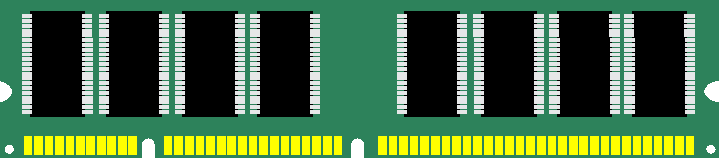
\includegraphics[height=0.3cm]{mem}} -- (3.45cm,-0.2cm) node[key]{memcached};
	\path (3.2cm,-1.1cm) node[anchor=east] (keybl) {
\includegraphics[height=0.9cm]{cvmfs}} -- (3.45cm,-1.1cm) node[key] (keybr) {CernVM-FS};
	\begin{pgfonlayer}{background}
        		\node[background, fit=(keytl) (keybl) (keybr)] {};
	\end{pgfonlayer}